\documentclass[11pt]{article}
\usepackage{graphicx}
\usepackage{listings}
\usepackage{anysize}
\renewcommand{\topfraction}{0.9}    % max fraction of floats at top
\renewcommand{\bottomfraction}{0.8}
\marginsize{2cm}{2cm}{1cm}{2cm}
\lstset{
  language=C,                     % choose the language of the code
}
\begin{document}

\title{Algorithms Coursework}
\author{Xueqi Chen and Haixiao Su}

\maketitle
\section{Add}
\begin{figure}[ht]
\centering
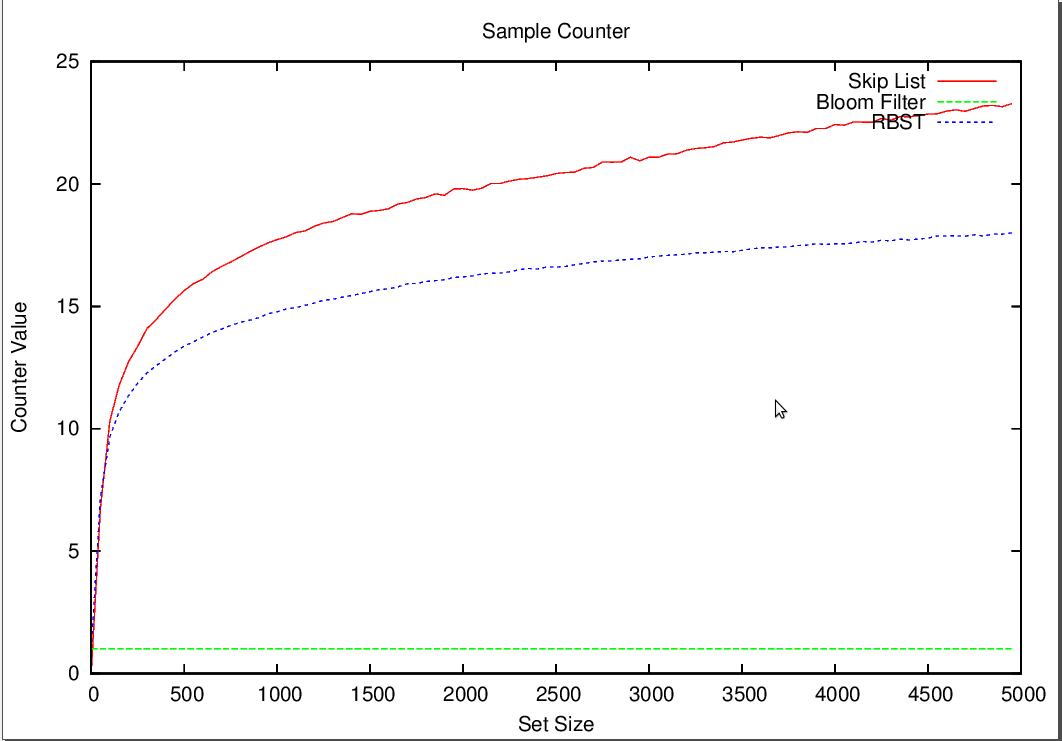
\includegraphics[height=70mm,width=100mm]{addcounter.png}
\caption{addcounter}
\end{figure}
\begin{figure}[ht]
\centering
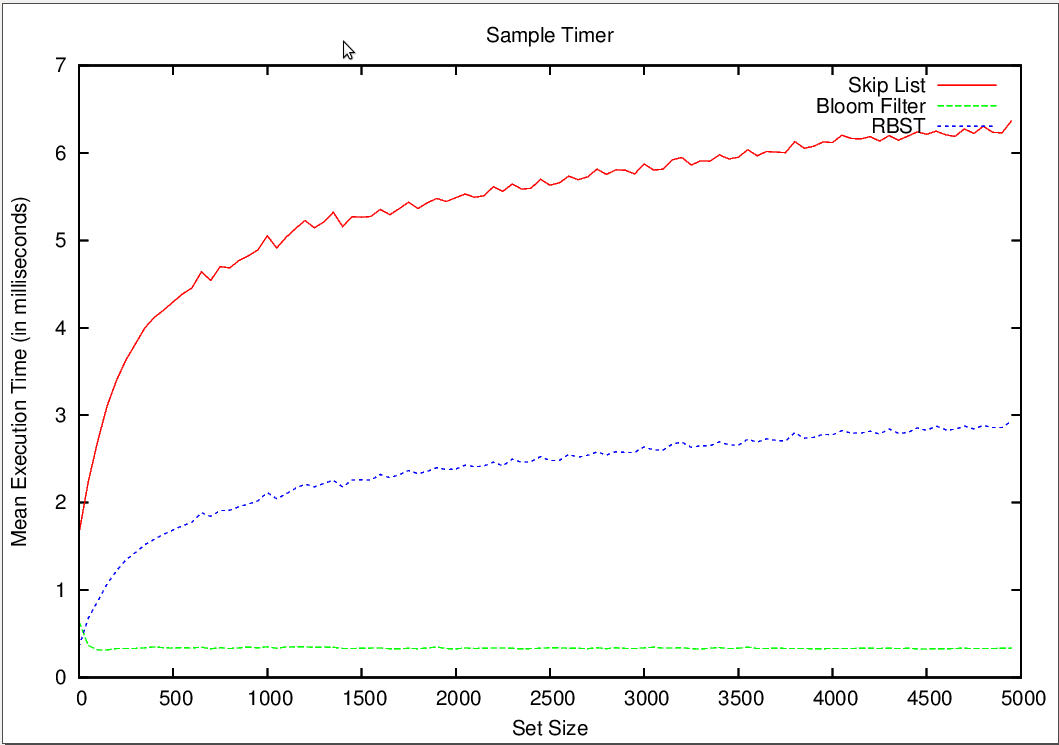
\includegraphics[height=70mm,width=100mm]{addtimer.png}
\caption{addtimer}
\end{figure}


\section{Delete}
\begin{figure}[ht]
\centering
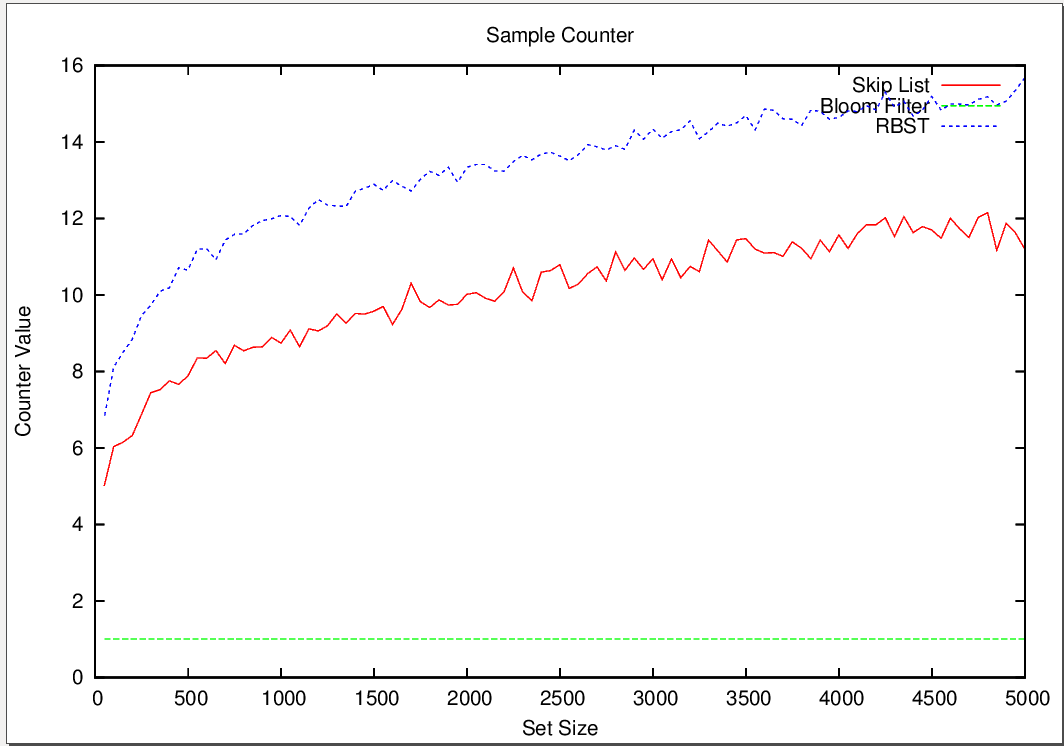
\includegraphics[height=70mm,width=100mm]{delcounter.png}
\caption{delcounter}
\end{figure}
\begin{figure}[ht]
\centering
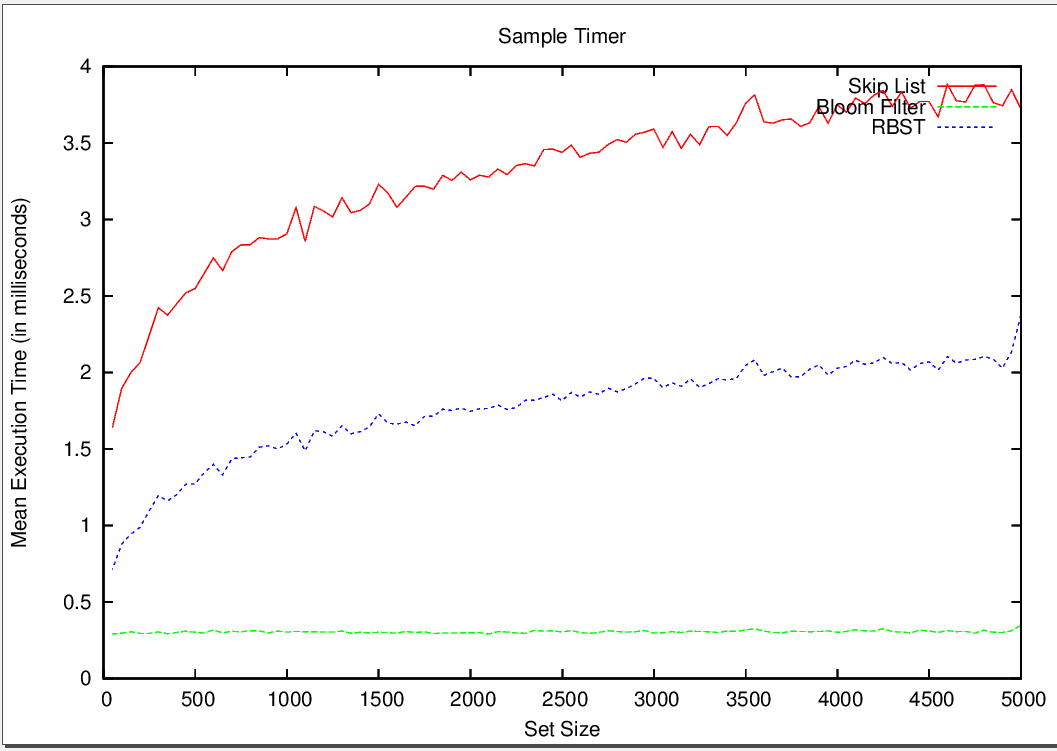
\includegraphics[height=70mm,width=100mm]{deltimer.png}
\caption{deltimer}
\end{figure}



\section{Find}
\begin{figure}[ht]
\centering
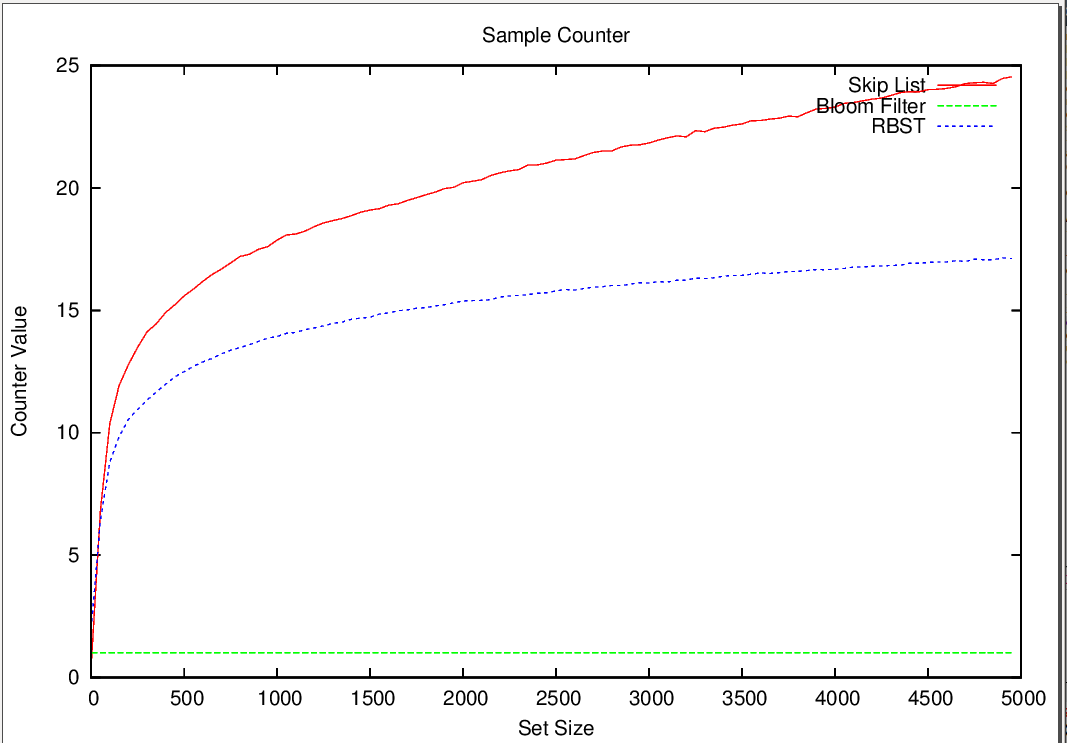
\includegraphics[height=70mm,width=100mm]{findcounter.png}
\caption{findcounter}
\end{figure}
\begin{figure}[ht]
\centering
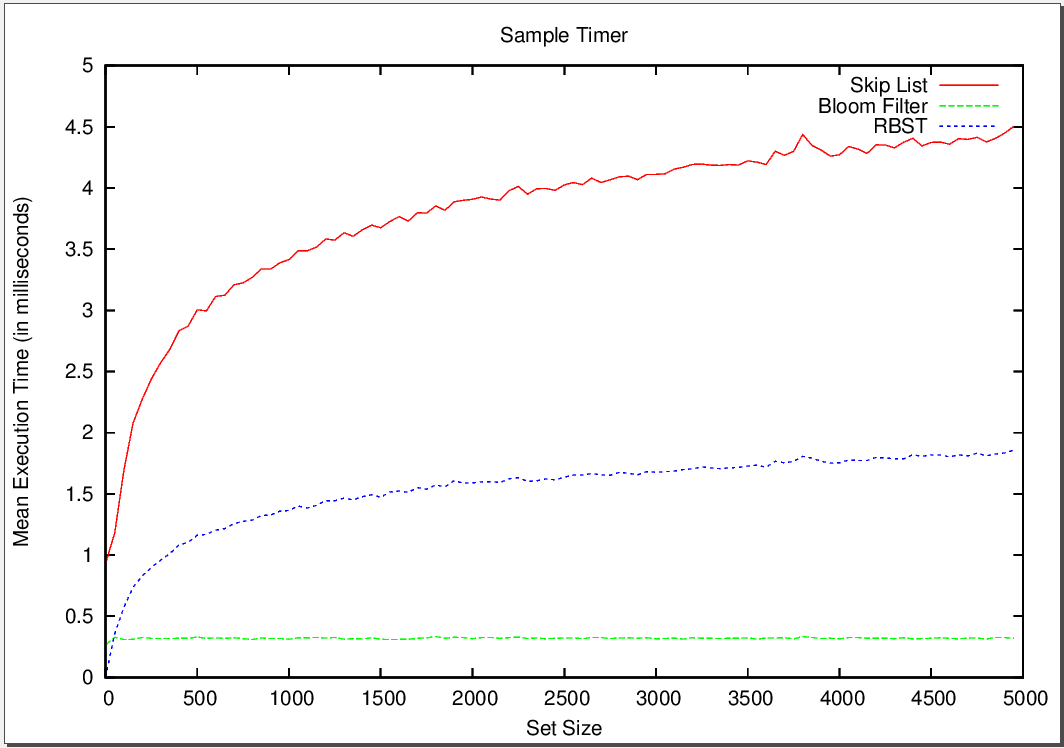
\includegraphics[height=70mm,width=100mm]{findtimer.png}
\caption{findtimer}
\end{figure}


\end{document}